%% Richard Wen
%% rwen@ryerson.ca


% *** INTRODUCTION ***


\section{Introduction} \label{introduction}

The wide availability of mobile devices have enabled millions of people to share online content, such as text, images, sound, and videos, from any location with wireless Internet connection. Social media platforms, such as Facebook \citep{Facebook:2017} and Twitter \citep{Twitter:2017}, are commonly used to share large amounts of online content in near real-time. This online content produces valuable sources of real-time locational data, known as geosocial media data, that may provide information on current real-world events such as traffic jams, natural disasters, disease spread, and terrorist attacks. Geosocial media data can be used to detect and predict real-world events given particular locations and times. However, human errors, inconsistencies, noise, high volumes, and constant changes make it difficult to extract useful information from geosocial media data. These issues cause a divide in the methods and approaches for geosocial media event detection and prediction, where standards, comparisons, and integration between different data sources and use cases are rare. This proposal documents a plan to develop a generalized framework and open source software for detecting and predicting real-world events using geosocial media data.

The objective of this proposal is to develop a framework and accompanying software to detect and predict real-world events in real-time with geosocial media data. A literature review was done to provide background knowledge on current research on event detection and prediction methods and applications. An approach, built on the knowledge from the literature review, was developed to satisfy the objectives. Recent progress was detailed to provide preliminary results and relevant past work related to the objectives. A discussion of the impacts was provided to address the importance and effect of the proposed research work.

The remaining sections are organized as follows:

\begin{itemize}
	\item \textbf{Section \ref{objectives}} details the objectives of the proposed research
	\item \textbf{Section \ref{literature-review}} provides a literature review of current research
	\item \textbf{Section \ref{approach}} details the proposed approach to satisfy the objectives and recent progress
	\item \textbf{Section \ref{conclusion-and-impact}} discusses the impact of the proposed research and provides concluding summaries and remarks
\end{itemize}

\section{Objectives} \label{objectives}

This section provides details objectives of this proposal. The main objective is to develop the following for detecting and predicting real-world events using geosocial media data:

\begin{enumerate}
	\item Framework that can be applied to a wide variety of applications and data
	\item Open Source Software based on (1)
\end{enumerate}

\subsection{Framework} \label{framework}

The framework objective requires that the following six components be identified and developed:

\begin{enumerate}
	\item \textbf{Data Sources}: Popular geosocial media platforms and data sources
	\item \textbf{Data Structures}: Geosocial media data structures
	\item \textbf{Event Detection Methods}: Common event detection methods and patterns
	\item \textbf{Event Prediction Methods}: Common event prediction methods and patterns
	\item \textbf{Output}: Resulting human-readable output information
	\item \textbf{Use Cases}: Common applications of geosocial media event detection and prediction
\end{enumerate}

\subsection{Software} \label{software}

The software objective requires that the following six open source components be identified and developed:

\begin{enumerate}
	\item \textbf{Databases}: Popular databases used for geosocial media data
	\item \textbf{Event Detection and Prediction Software}: Libraries or packages for event detection and prediction algorithms and models
	\item \textbf{Information Software}: Libraries or packages for displaying and extracting information from model outputs
	\item \textbf{Online Platform}: Online websites to host and distribute software
	\item \textbf{Testing Software}: Libraries or packages to conduct standard unit tests
	\item \textbf{Documentation Software}: Libraries or packages to document software for a wide audience
\end{enumerate}


% *** LITERATURE REVIEW ***


\section{Literature Review} \label{literature-review}

This section provides a literature review to provide background knowledge on current research related to the topic of \textit{"real-time geosocial media event detection and prediction"}. Papers were selected from the Association for Computing Machinery (ACM) and Institute of Electrical and Electronics Engineers (IEEE) Xplore digital libraries. Figure \ref{figure:papers_yearly} shows  the distribution of selected papers for review by year. Appendix \ref{appendix:literature-review-methods} provides details of the methods used for paper selection and review.

\begin{figure}[!htb]
\begin{center}
\begin{tikzpicture}
\begin{axis}[
	ylabel=Papers,
	xlabel=Year,
	ybar interval=1,
	xticklabel style={/pgf/number format/1000 sep=,}
	]
	\addplot[color=gray, fill=black] table[x=year, y=papers] {data/papers_yearly.tsv};
	\legend{}
\end{axis}
\end{tikzpicture}
\caption{\textbf{ACM and IEEE Published Papers Found from 2012 to December 2, 2017.} A total of 22 papers were reviewed. Black bars represent the selected papers filtered from the potential papers using the literature review methods described in Appendix \ref{appendix:literature-review-methods}.}
\label{figure:papers_yearly}
\end{center}
\end{figure}

\subsection{Event Detection and Prediction} \label{event-detection}

 Event detection and prediction methods using geosocial media data are focused on statistical, machine learning, clustering, and network based approaches. \cite{Alvanaki:2012} use sliding time windows to compute statistics about social media tags in order to detect unusual correlation shifts that are probable emergent topic events. \cite{Khabiri:2012} used closeness measures, term selection, and dynamic sliding windows to annotate social media messages with informative and more abstract terms, however the techniques used were infeasible for real-time annotation when smoothing was implemented in the sliding windows. \cite{Sofean:2012} used machine learning methods to classify medical-related tweets on Twitter based on world topics relative to diseases and symptoms. \cite{Middleton:2014} suggested the use of re-tweets from Twitter for credibility measures, and context filters to narrow natural disaster events to specific classes such as positive, negative, or urgent reports with natural language text. \cite{Hazra:2015} built a web application with event sockets that extracted news-worthy Twitter events, which can be personalized to particular interests, but machine learning may be needed improve the user recommendation system, and historical events were not considered. \cite{Enoki:2015} used in-memory stores for real-time topic querying given social diffusion of popular Twitter messages. \cite{Abrol:2015} used cloud computing to profile and geo-locate millions of users for social behavioural patterns, changes, and events in real-time, but required improvements to handle simultaneously emerging new classifications. \cite{Buntain:2015} used social media features such as location and metadata to evaluate the credibility of detected events. \cite{Buntain:2016} used a technique which identified rapid increases in social media posts to detect events and improve the performance of other real-time tracking systems. \cite{Lee:2017} used machine learning methods to extract important word features from social media data to predict flu activity 2 to 3 weeks ahead in real-time. \cite{Li:2017} used semantic and similarity clustering to identify old and new geosocial media events with the same meaning in real-time. \cite{Tsikerdekis:2017} compared several optimization techniques to reduce the volume or velocity of social media data for identity deception detection, and concluded that data velocity is a major factor in considering detection methods. A majority of the methods presented in the literature focused on geosocial media event detection methods, but few mentioned or considered event prediction in real-time.

\subsection{Visualization} \label{visualization}

After detecting or predicting geosocial media events, the model outputs must be visualized into human-understandable information to appropriately act and respond to each event. \cite{Zubiaga:2012} used summarization techniques to reduce the large volume of Twitter data to provide a higher level  textual abstraction of social media events and topics. \cite{Calderon:2014} designed streaming graphs to visualize real-time Twitter sentiments for emergency management, where a study on 21 randomy selected participants concluded that visualization of real-time social media data required interactive interfaces, geo-location context, and human cognition and reasoning theory. \cite{Middleton:2014} mapped real-time social media data using textual geo-parsing, spatial clustering, and a combination of various data sources, such as Volunteered Geographic Information (VGI), online mapping services, and gazetteers, to visually display areas of potential events. \cite{Xia:2014} developed a web-based visualization, consisting of a web map with complementary photos and graphs, for multiple social media sources such as Instagram, Twitter, and Foursquare to provide real-time events and news trends for a city. \cite{Tsirakis:2015} created a web-based dashboard application that displays the current trending events, influential users, and popular topics in real-time, but had considerations with the scalability of algorithms, multiple data sources, and language integrations. \cite{Shah:2015} used background knowledge from Wikipedia to summarize social media events relative to photos and videos in real-time. \cite{Kumar:2016} used nodes to represent social media users for creating visual networks of Twitter users to analyze and detect the strength of social relationships among users. \cite{Wang:2017} used natural language processing techniques to detect traffic incidents for a real-time traffic alerts and warnings system. The majority of the visualization approaches proposed in the literature involved interactive, web-based, interfaces that transformed lower level details of model results into higher level abstract visuals to produce human-understandable information.

\subsection{Applications} \label{applications}

Event detection and prediction methods are widely used for real-world applications related to the categories of disaster, disease, travel, and the environment. Figure \ref{figure:papers_applications} shows the number of papers in each category from the literature. \cite{Sofean:2012} created a real-time surveillance architecture to detect disease-related social media postings on Twitter. \cite{Riga:2014} used machine learning models to cluster Twitter tweets for urban air quality monitoring and soft sensing. \cite{Middleton:2014} used geosocial media event detection to obtain real-time crisis maps and reports for hurricanes and earthquakes in disaster response. \cite{Semwal:2015} used machine learning techniques to detect and predict daily co-occurring traffic event issues with social media data. \cite{Bodnar:2017} used social media data together with electrical consumption data to discover relevant energy-related topics and to gain real-time insight on energy consumption of users in urban areas. \cite{Lee:2017} used geosocial media data with historical diseases datasets to predict future influenza events in real-time. The majority of the papers in the literature conducted experiments and tests in disaster applications, followed by disease, travel, and environment in order.

\begin{figure}[!htb]
\begin{center}
\begin{tikzpicture}
\begin{axis}[
	xbar interval=1,
	xlabel=Papers,
	xtick={0,1,2,3,4,5,6,7},
	ytick=data,
	yticklabels={Environment, Travel, Disease, Disaster}
	]
	\addplot[color=gray, fill=black] table[y=code, x=papers] {data/papers_applications.tsv};
	\legend{}
\end{axis}
\end{tikzpicture}
\caption{\textbf{Applications in ACM and IEEE Published Papers from 2012 to December 2, 2017.} Disease refers to human health-related disease spread events. Disaster refers to natural disasters and human-related emergencies. Environment refers to environmental-related applications such as air pollution and urban energy utility. Travel refers to vehicular traffic and transportation related applications. Black bars represent the number of papers in each application category, where papers were selected using the literature review methods in Appendix \ref{appendix:literature-review-methods}.}
\label{figure:papers_applications}
\end{center}
\end{figure}


% *** APPROACH ***


\section{Approach} \label{approach}

This section provides details on the methods for  the proposed approach and milestones to achieve the research objectives. Recent progress toward the objectives is also mentioned in this section.

\subsection{Methods} \label{methods}

The proposed methods to achieve the research objectives involve first developing a geosocial media event detection and prediction framework, followed by the development of openly-accessible software based on that framework to create real-time systems in practice. In order to develop the framework, commonly used data, techniques, and methods for event detection and prediction will be further reviewed using research literature to satisfy the six components from the framework objectives in Section \ref{framework}. Figure \ref{figure:framework} shows the dependency between the different framework components. The data sources will determine the data structures, which will determine the event prediction and detection methods. The event prediction and detection methods will then determine the model output results and the potential use cases and applications. The framework will be the abstract representation used to develop the practical geosocial media event detection and prediction software for building real-time systems. The software development will consist of selecting open source software libraries and packages to satisfy each of the framework's identified components to create a modular system that can adapt to different real-world applications and geosocial media sources. The proposed approach will be to identify each framework component in dependent order starting from the data sources component. After identifying a component, software will be developed for that particular component individually, which enables it to work without reliance on other components. Connecting software will then be developed between each component to enable interoperability. The software development approach is shown in Figure \ref{figure:software}.

\begin{figure}[!htb]
	\centering
	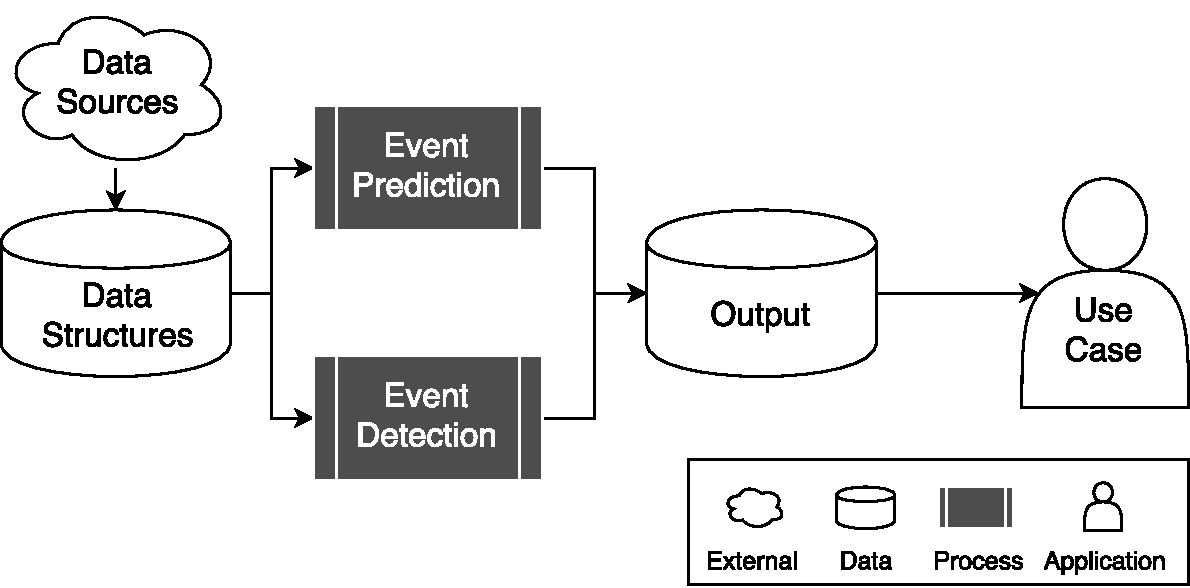
\includegraphics[width=6in]{framework}
	\caption{\textbf{Framework Components Dependency.} The framework seeks to group components in the multiple detection and prediction methods reviewed in the literature to form a standardized and more consistent approach that is flexible, adaptable, and comparable among different implementations.}
	\label{figure:framework}
\end{figure}

\begin{figure}[!htb]
	\centering
	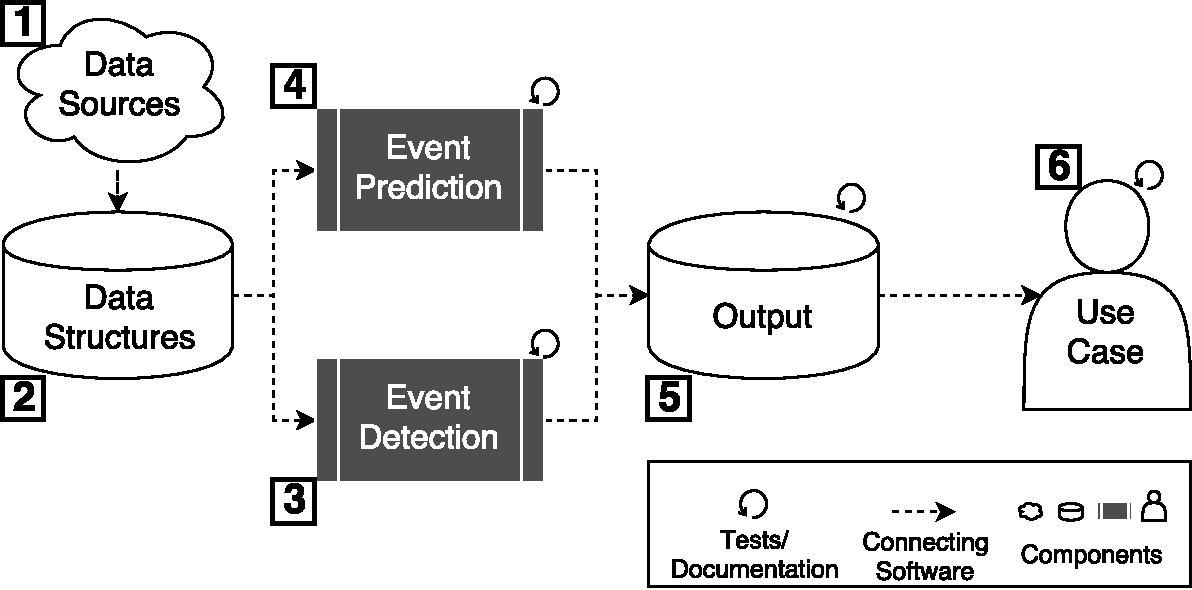
\includegraphics[width=6in]{software}
	\caption{\textbf{Software Components Development Approach.} Each number represents an ordered step and milestone in the software development approach that will be conducted after the identification of the relevant framework component. The connecting software is used to integrate multiple components together, but each component is tested and documented individually first as smaller parts to a whole.}
	\label{figure:software}
\end{figure}

\subsection{Recent Progress} \label{recent-progress}

Recent progress involved the partial identification of several framework components and development of a small software package. The identified framework and software components are provided in Table \ref{table:frameworkcomponents} and \ref{table:softwarecomponents} respectively. A small software package was developed for Node.js \citep{Nodejs:2017} named \textit{"twitter2pg"}  \citep{Wen:2017} to conveniently extract real-time Twitter data into a relational PostgreSQL database \citep{Postgresql:2017}. The package has been downloaded 259 times as of December 2, 2017 after approximately a month of release, and consists of documentation, unit tests, and automatic Linux builds for continuous tests every month.

\begin{table}[!htb]
\centering
\caption{\textbf{Identified Framework Objective Components.}}
\label{table:frameworkcomponents}
\begin{tabular}{|p{2.5in}|p{3.5in}|}
\hline
\textbf{Component} & \textbf{Identified}\\
\hline
Data Sources & Twitter Streaming API, Programmable Web\\
\hline
Data Structures & Unstructured (JSON), Location Points, Time Stamp \\
\hline
Event Detection Methods & Frequency, Sliding Window, Normalization, Clustering, Sampling, Graphs, Machine Learning\\
\hline
Output & Textual Summary, Webmap, Wordcloud\\
\hline
Use Cases & Influenza, Earthquake, Psychosocial, Energy, Traffic, Air Quality\\
\hline
\end{tabular}
\end{table}

\begin{table}[!htb]
\centering
\caption{\textbf{Identified Software Objective Components.}}
\label{table:softwarecomponents}
\begin{tabular}{|p{2.5in}|p{3.5in}|}
\hline
\textbf{Component} & \textbf{Identified}\\
\hline
Databases & PostgreSQL, MongoDB, MySQL, Hbase, Cassandra, Accumulo, GeoMesa\\
\hline
Event Detection and Prediction Software & Massive Online Analysis (MOA), scikit-learn, Apache Spark, Apache Kafka\\
\hline
Information Software & Leaflet, Carto, D3.js\\
\hline
Online Platform & Github, PyPi, npm\\
\hline
Testing Software & travis Continuous Integration (CI), Docker\\
\hline
Documentation Software & HTML, Markdown\\
\hline
\end{tabular}
\end{table}


% *** CONCLUSION AND IMPACT ***


\section{Conclusion and Impact} \label{conclusion-and-impact}

This proposal presented a potential framework and accompanying software for geosocial media event detection and prediction based on current research. The framework was proposed to provide a more consistent approach to working with geosocial media data, and to more easily allow non-experts to have a standard solution for a wide variety of applications such as traffic management, disease control, and disaster response. The impacts of a framework and software for geosocial media event detection and prediction are related to approach consistency improvements, standardized solutions, and transparency in geosocial media event-based systems research. The proposed framework seeks to standardize and reduce the inconsistency of approaches in different areas of geosocial media event detection and prediction applications. It provides a common approach that guides the user in constructing a real-time system for event detection and prediction, and allows for comparability between different implementations. The proposed open source software provides an openly-accessible and transparent solution to creating real-time event detection systems in practice. It will adequately address common issue in developing real-time event detection and prediction systems with geosocial media data, and enable practitioners to more easily create systems for particular use cases in the real-world. The major contributions of the proposed research is then a flexible and adaptable framework for real-time geosocial event detection and prediction, followed by accompanying software for use in practice.

